
\section{Single Agent Approach}

The goal of this section was to design a system that fulfilled the requirements outlined in Problem~\ref{prob:sub2}

The general shape of a GA as seen in Algorithm~\ref{alg:GenericGA} is the same for almost all problems. But each individual operator implementation is domain specific.

\subsection{Individual Encoding}
As such, I first had to implement a method to generate an initial population. In order to do this, I had to define my programmatic representations of the phenotypes and genotypes of my individuals. I decided to base my pheno and genotypic structure on the that described by Kala\cite{kalaOnroadIntelligentVehicles2016}.

In this approach, the phenotype is abstractly represented as a Bézier curve (Section~\ref{sec:back-bezier-curves}). This is more concretely translated into a genotype encoded as a real-valued string, interleaving the $x$ and $y$ coordinates of each control point. Taking the form:

\begin{figure}[ht]
	\centering
	\begin{tikzpicture}[
			block/.style={minimum height=2.2em,outer sep=0pt,draw,rectangle,node distance=0pt}]

		\node [block] (A) {$P_{0_{x}}$};
		\node [block, right = of A] (B) {$P_{0_{y}}$};
		\node [block, right = of B] (C) {$P_{1_{x}}$};
		\node [block, right = of C] (D) {$P_{1_{y}}$};
		\node [block, right = of D] (E) {$\ldots$};
		\node [block, right = of E] (F) {$P_{n_{x}}$};
		\node [block, right = of F] (G) {$P_{n_{y}}$};

	\end{tikzpicture}
	\caption{\label{fig:GA_Genotype} Individual genotype as real-valued string }
\end{figure}

In the above form the descriptions of genetic operators found in Section~\ref{subsec:GAOps} should be sufficiently detailed to re-implement.
\todo[inline]{Replace with detailed description of implementation of operators, decisions e.g. allowed range for mutation of control points.}

Initially my Phenotype contained no additional information. However, I still created the distinction to allow for additional properties to be encapsulated during development.

\subsection{Population Generation}

Population generation theoretically can be very simple and generate very little diversity, relying on the other operators to explore the search space. However, the more diverse a set of initial routes one can generate, the quicker the system will converge to an optimal solution.

As such we want to ensure that both the number of control points as well as their position are properly varied.

The first and last control points \textbf{must} be the starting and goal position for the agent. In a Bézier curve these are the only two points that the curve definitely passes through. We must also ensure that the $x$ coordinates of the control points are in order, so as to avoid routes which \textit{double back} on themselves. This can also occur as the result of other operators such as crossover and mutation, we can fix this using a simple repair operator which re-orders points based on their $x$ positions.

Once the initial population is generated, the main algorithmic loop can begin, this is the repeated application of the selection, crossover, mutation and evaluation operators (See Section~\ref{subsec:GAOps}) until set termination criteria are met or the maximum number of generations is completed, seen in Algorithm~\ref{alg:GenericGA}.

\subsection{Fitness assessment}

\todo[inline]{Have I actually explicitly stated the construction of my fitness function \& referenced Kala for inspiration?}


The foundation of my Fitness function is the length of each route, i.e. the length of a given $n$ degree Bézier curve. This calculation can be accurately approximated using Equation~\ref{eq:bezlength} as the true calculation is expensive and does not generalise nicely to $n$ degrees\cite{gravesenAdaptiveSubdivisionLength1997}.

Minimising the length of a route is a good way of ensuring generated routes are direct, however, other values and heuristics are required to maintain other requirements such as to make sure changes in direction are not too severe or that a route does not pass through infeasible space (avoiding obstacles etc.).

\subsubsection{Road Section Definition}

I initially experimented with an alternative coordinate space which enabled me to completely enclose the search space within the area of the road, eliminating the possibility of generating routes that left the \textit{road}. This was inspired by the ``Road coordinate axis system'' described by Kala in~\cite{kalaOptimizationBasedPlanning2016}. However I abandoned this concept as it did not appear to increase performance and introduced overhead when visualising or generating the routes.

Instead I defined each section of road using the following Structure:

\begin{minted}{julia}
struct Road
    boundary_1::Function
    boundary_2::Function
    obstacles::Array{Obstacle}
    length::Real
end
\end{minted}

This approach allows me to define the upper and lower boundary of a road as any function, straight roads can be defined as a pair of straight lines a certain width apart, and arbitrarily complex roads can be represented using arbitrarily complicated functions.

For example the road seen in Figure~\ref{fig:simple-road} had boundary functions:

\begin{align*}
  b_{1}(x) &= 0 \\
  b_{2}(x) &= 5
\end{align*}

And the curved road section seen in Figure~\ref{fig:curved-road} functions:

\begin{align*}
  b_{1}(x) &= 2\cosh (0.1x)-2 \\
  b_{2}(x) &= 2\cosh(0.12x)+8
\end{align*}

Where in both cases the length of the road (and therefore upper bound of $x$) was 25, the lower bound of $x$ was 0.

\begin{figure}[ht]
  \centering
  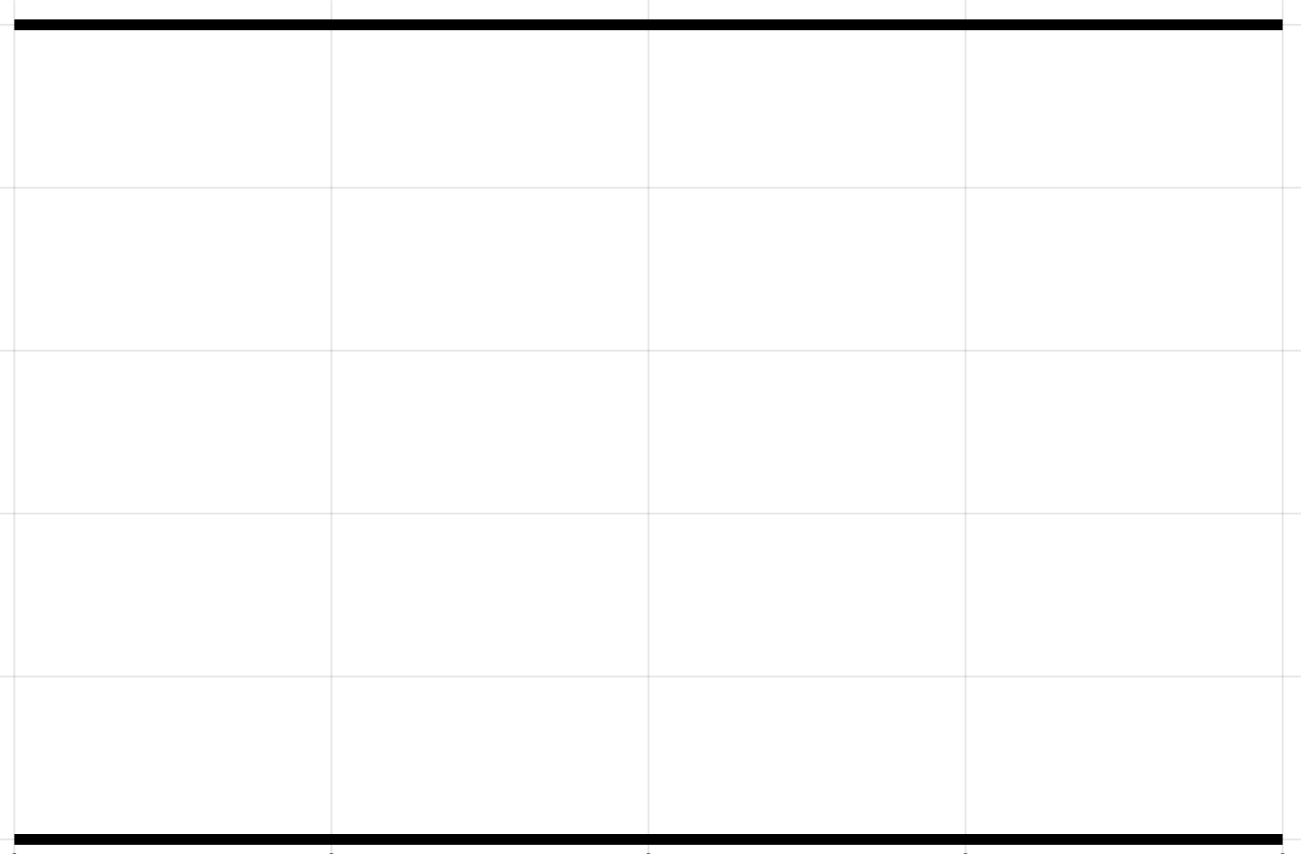
\includegraphics[scale=0.2]{figures/simple-road.png}
  \caption{\label{fig:simple-road} A straight road}
\end{figure}

\begin{figure}[ht]
  \centering
  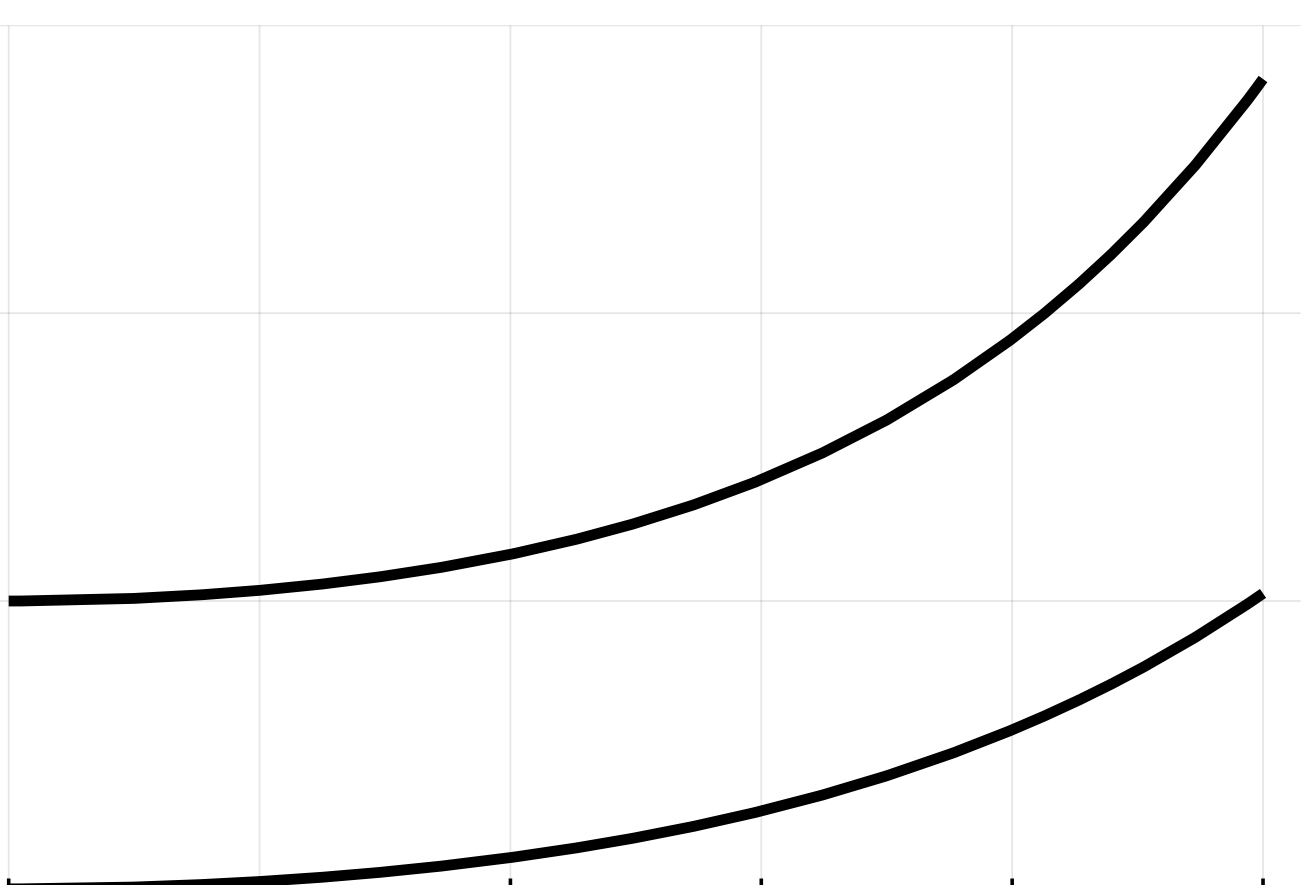
\includegraphics[scale=0.2]{figures/curved-road.png}
  \caption{\label{fig:curved-road} A curved road}
\end{figure}

\paragraph{Road Obstacles}

I have implemented two basic \texttt{Obstacle} types (\texttt{Rectangle} and \texttt{Circle}) allowing me to create regions of infeasible space within the valid road-space.

Infeasible space is then calculated by taking a sample of 500 points along a given curve $B$ and checking which (if any) lie within any of the obstacles.

A Bézier curve is then constructed using two applications of De Casteljau's algorithm (See Section~\ref{sec:decasteljau}) using values for $t$ derived from the subsample points. An illustration of this process can be seen in Figure~\ref{fig:ifspace-illustration}. The length of this curve is weighted and added to the overall fitness of the candidate solution. The stages progress as Follows:

\begin{enumerate}
  \item Curve and obstacle drawn
  \item Uniform sample of points chosen along curve
  \item Curve segment from origin to first infeasible point isolated
  \item Curve segment from last infeasible point to end position isolated
  \item Infeasible distance calculated as difference in length between original curve and two isolated segments
\end{enumerate}


A similar process is performed to determine how much of a curve passes too closely to an infeasible region, this is penalised with a separate, lower, weighting.

\begin{figure}
  \centering
  \begin{subfigure}[b]{0.44\textwidth}
    \centering
    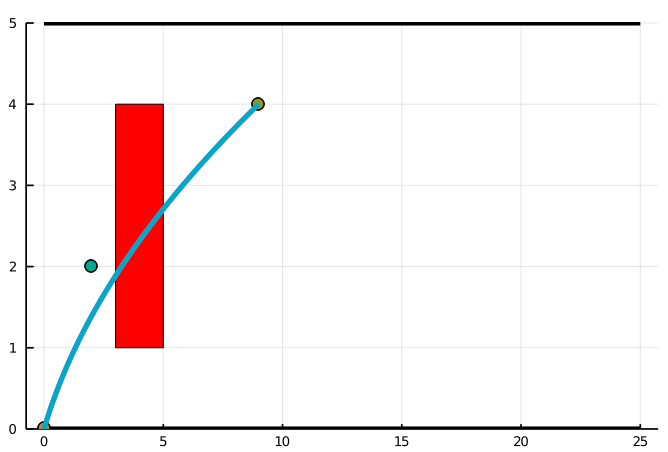
\includegraphics[width=\textwidth]{figures/obstacleavoidance-stage1.png}
    \caption{Stage 1}
  \end{subfigure}
  \begin{subfigure}[b]{0.44\textwidth}
    \centering
    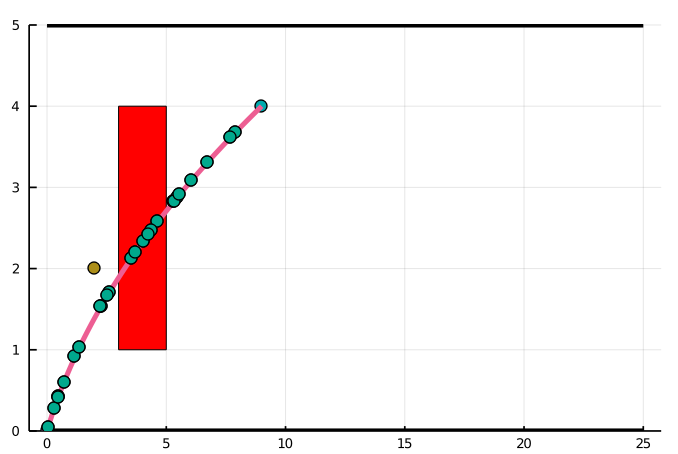
\includegraphics[width=\textwidth]{figures/obstacleavoidance-stage2.png}
    \caption{Stage 2}
  \end{subfigure}
  \begin{subfigure}[b]{0.44\textwidth}
    \centering
    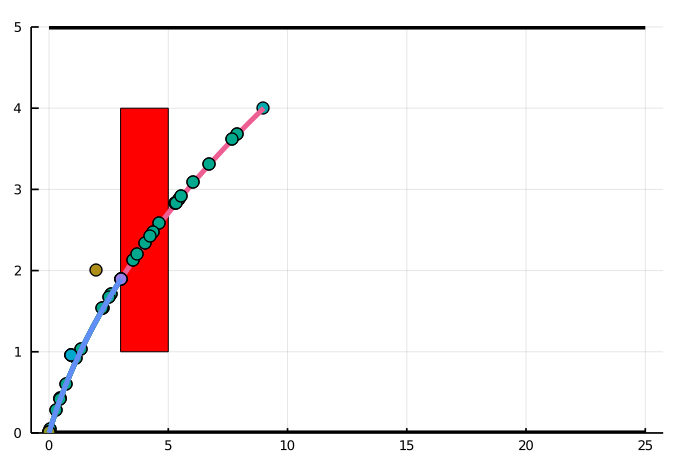
\includegraphics[width=\textwidth]{figures/obstacleavoidance-stage3.png}
    \caption{Stage 3}
  \end{subfigure}
  \begin{subfigure}[b]{0.44\textwidth}
    \centering
    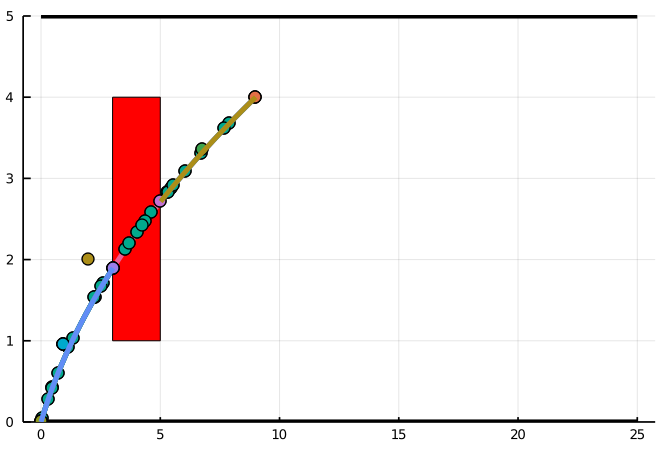
\includegraphics[width=\textwidth]{figures/obstacleavoidance-stage4.png}
    \caption{Stage 4}
  \end{subfigure}
  \begin{subfigure}[b]{0.44\textwidth}
    \centering
    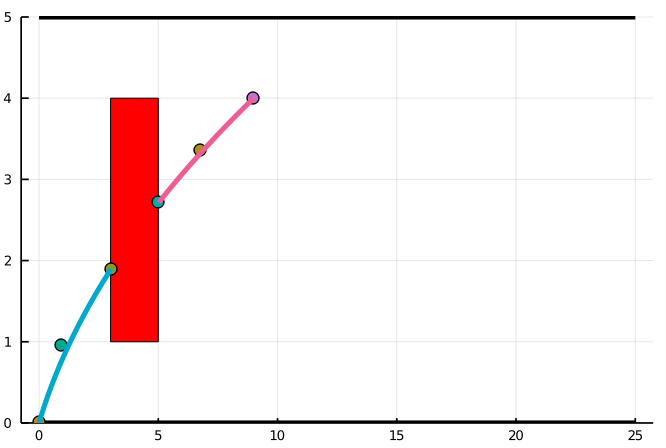
\includegraphics[width=\textwidth]{figures/obstacleavoidance-stage4-aux.png}
    \caption{Stage 5}
  \end{subfigure}
  \caption{\label{fig:ifspace-illustration} Illustration of finding infeasible section of curve}
\end{figure}\todo[inline]{Technically this infeasible distance calculation has very slightly changed in implementation, is it worth redoing or just leave as is?}

Now with the ability to calculate the length of a route as well as the distance it travels through/ too close to infeasible space, I can define my Fitness function:

\begin{multline}\label{eq:basefitness}
  \mathcal{F}(i) = \\
  L_{i} +\\
  \alpha \cdot \texttt{infeasible distance}(i) + \beta \cdot \texttt{high-proximity distance}(i)
\end{multline}\todo{formatting}

Where:
\begin{itemize}
  \item $L_{i}$ is the length of candidate $i$'s route
  \item \(\alpha\) and \(\beta\) are weighting parameters s.t.

        $\alpha > \beta > 1$

        therefore penalising infeasible distance harder than distance which is \textit{too close} to infeasible space, guiding the GA to prioritise avoiding infeasible space.
\end{itemize}

This function is inspired by Kala\cite{kalaOptimizationBasedPlanning2016} and proves to be a good basis for a naive single agent planner, futher augmentation is required to support multiple agents or variable velocity profiles.


\subsection{Genetic Operators}

The abstract goal of each genetic operator has already been discussed in Section~\ref{subsec:GAOps}. Here I will discuss their concrete implementation with respect to my task.

\subsubsection{Selection}
\label{subsec:approach:selection}

My selection procedure follows very closely to the method outlined in Section~\ref{subsec:GAOps}, relying on the fitness function to duplicate fit individuals, replacing the less fit ones with a certain chance or reasoning.

An example of ranked selection on a sample population can be seen in Figure~\ref{fig:selection_eg}

\begin{figure}
  \centering
  \begin{subfigure}[b]{0.44\textwidth}
    \centering
    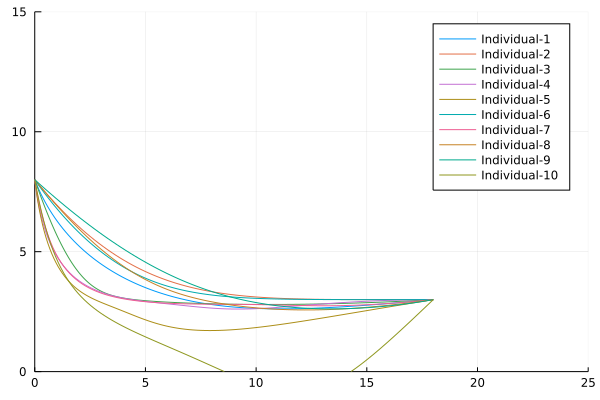
\includegraphics[width=\textwidth]{figures/init_pop.png}
    \caption{Initially generated population, size 10}
  \end{subfigure}
  \begin{subfigure}[b]{0.44\textwidth}
    \centering
    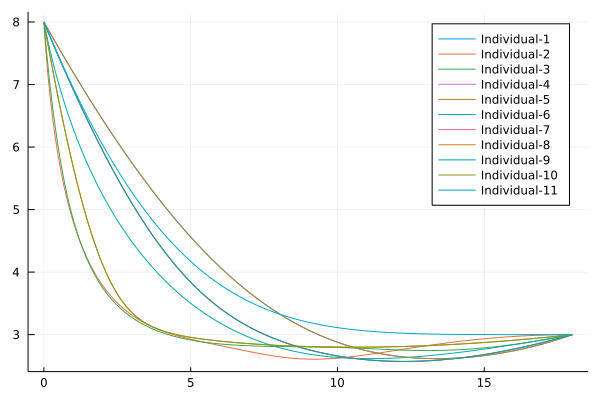
\includegraphics[width=\textwidth]{figures/post_selection_pop.png}
    \caption{Population after (ranked) selection procedure}
  \end{subfigure}
  \begin{subfigure}[b]{0.44\textwidth}
    \centering
    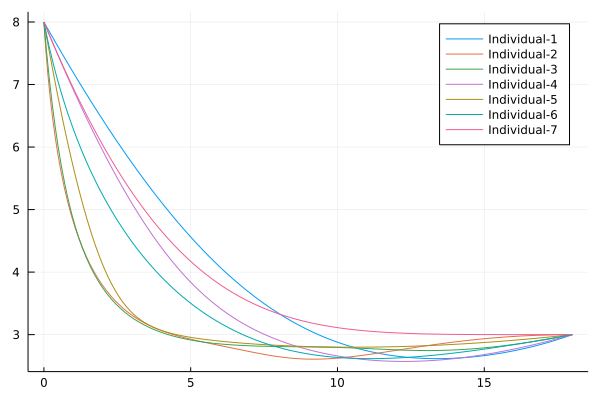
\includegraphics[width=\textwidth]{figures/post_selection_pop_unique.png}
    \caption{Population after (ranked) selection procedure, duplicates removed}
  \end{subfigure}
  \caption{\label{fig:selection_eg} Example of ranked selection}
\end{figure}


\subsubsection{Mutation}

The variants of the mutation operator that I have implemented are Uniform and Gaussian. Both attempt to achieve the same effect via different methods.

Abstractly, my mutation operators select a control point with a random probability and mutate within fixed bounds. These bounds are tied to the size and shape of the road.

In my Gaussian mutation operator, the range of $x$ values for the mutation of a randomly selected point $ p \in B = \{ p_{1}, \ldots, p_{n} \}, n\in \mathbb{Z}^{\geq 2 }$ are:

\begin{equation}
\mathcal{X} = \left[p_{1_{x}}, p_{n_{x}}\right], p_{1}, p_{n} \in B
\end{equation}

I.e. a mutated control point cannot lie before or after the start or end points respectively. The range of $y$ values a mutated point can take is within:

\begin{equation}
  \mathcal{Y} = \left[ - 1.3 \cdot \frac{b_{1}(\mathcal{X}_{1}) + b_{2}(\mathcal{X}_{2})}{2}, 1.3 \cdot \frac{b_{2}(\mathcal{X}_{1}) + b_{2}(\mathcal{X}_{2})}{2} \right]
\end{equation}

Meaning $-1.3$ times the average $y$ coordinate of the bottom road boundary to $1.3$ times the average of the top road boundary across the range of permitted $x$ values. $\pm 1.3$ was used after experimenting with values ranging from $\pm 2$ to $\pm 0.5$, 1.3 offers the procedure the chance to significantly affect the course of a route whilst, minimising the chance that the mutated route will be infeasible.

A pair standard deviations as previously outlined in the Background section are defined as:

\begin{equation}
\sigma_{x} = \frac{\mathcal{X}_{1}-\mathcal{X}_{2}}{10}
\end{equation}

\begin{equation}
\sigma_{y} = \frac{\mathcal{Y}_{1}-\mathcal{Y}_{2}}{10}
\end{equation}

A new point, $p'$, is then constructed as follows:

\begin{align}
  p'_{x}  &= \min(\max(\mathcal{N}(p_{x},\sigma_{x}),\mathcal{X}_{1}),\mathcal{X}_{2})\\
  p'_{y}  &= \min(\max(\mathcal{N}(p_{y},\sigma_{y}),\mathcal{Y}_{1}),\mathcal{Y}_{2})
\end{align}

Point $p \in B$ is then replaced with our new point $p'$.

The result of the operation being applied to a example curve can be seen in Figure~\ref{fig:gauss_mutation_eg}

\todo{Talk about implmentation of Uniform mutation operator }

\begin{figure}[ht]
  \centering
  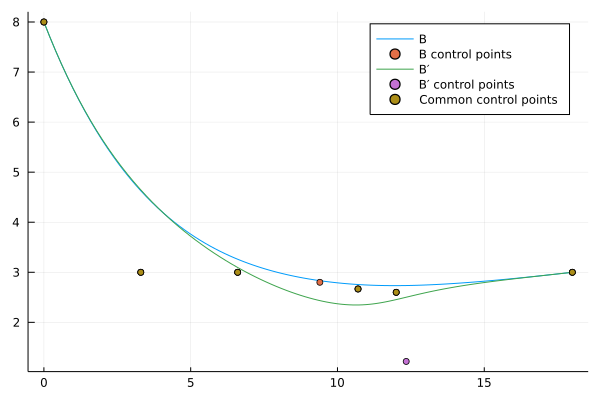
\includegraphics[scale=0.4]{figures/gauss_mutation_eg.png}
  \caption{\label{fig:gauss_mutation_eg} Example of Gaussian mutation on a Bézier curve}
\end{figure}

\subsubsection{Crossover}

Simple crossover is implemented as it is described in Section~\ref{subsec:GAOps}, two parents are randomly selected and exchange genotypic information about a random point. I have been careful not to choose a crossover point which splits a control point. The result of this operation is appended to the current population, only the top $n$ individuals are carried forward to the next generation.
Once used to create offspring, an individual cannot again participate in crossover, however, duplicate individuals created via the selection process may effectively reproduce multiple times.

The result of a single (simple) crossover operation can be seen in Figure~\ref{fig:crossover_eg}

\begin{figure}
  \centering
  \begin{subfigure}[b]{0.44\textwidth}
    \centering
    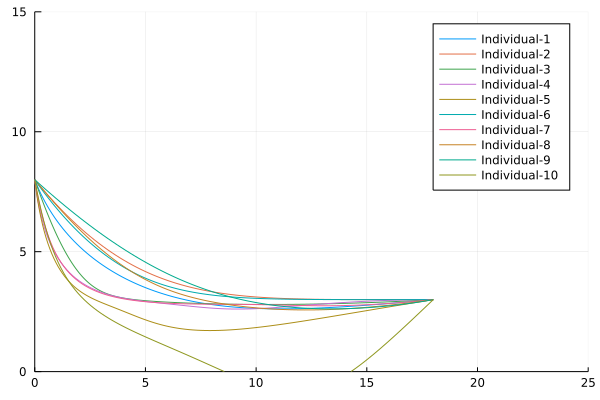
\includegraphics[width=\textwidth]{figures/init_pop.png}
    \caption{Initially generated population, size 10}
  \end{subfigure}
  \begin{subfigure}[b]{0.44\textwidth}
    \centering
    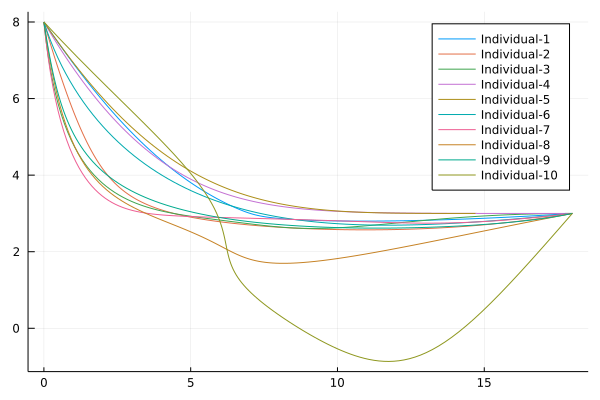
\includegraphics[width=\textwidth]{figures/post_crossover_pop.png}
    \caption{Population after crossover operation is applied}
  \end{subfigure}
  \caption{\label{fig:crossover_eg} Example of simple crossover}
\end{figure}

\section{Multi-agent Approach}
\label{sec:maa}

So far we have only concerned ourselves with planning a route through a road-space for a single agent. However, in the real world, roads are seldom occupied by a single vehicle and as such we must consider how to efficiently plan a set of routes for a set of agents between between a set of coordinate pairs, such that, our agents do not collide at any point in time.

There are different approaches we can take to this problem. \todo[inline]{refer to lit rev sections discussing approaches by Kala\cite{kalaOnroadIntelligentVehicles2016} and Cai \& Peng \cite{caiCooperativeCoevolutionaryAdaptive2002}}

My initial approach \todo{refer to ?Cai+Peng? as their approach was similar} to a collaborative planning system was somewhat inefficient. The system operated by planning routes for each agent sequentially, using a growing \textit{context} to keep track of the routes that had already been finalised. The first agent to be planned was not concerned with avoiding collisions, because, as far as it was concerned, there were no other agents in the system. Each subsequent agent checked if any of its candidate solutions intersected with any of the routes planned before, a very high penalty was applied to any routes with collisions.

This system was very inefficient with the final routes requiring a large number of checks to be carried out by my \texttt{bezInt} function, which itself suffered from \todo[inline]{verify this} exponential time (and space) complexity.

This system was improved upon by splitting the process over multiple threads, each agent being given a separate thread, communicating their most up-to-date plans via a shared array, $S$. Agent $i$ will store its current fittest route in $S[i]$, the calculation for fitness of any candidate checks for collisions with each route in $S$. This system may conduct more checks but it removes the problem of prioritising the first route to be planned and reduces the overall runtime of the system approximately proportionally to the number of threads available, an abstract view of the topology can be seen in Figure~\ref{fig:PCGA} with each agent $a_{k}, k \in [1,n]$ being mapped to a separate threaded instance of my GA planner. Each instance has access to the shared array which stores the fittest route after generation $i \in [1,m]$ with $m$ being the maximum number of generations for each agent.

Updates to the shared array happen as and when each thread reaches the end of a generation. This can mean that routes that terminate before others have to adapt less to other routes, but this trade-off cannot be avoided without instituting constant communication between threads, which in and of itself introduces overhead and slows down planning.

\begin{figure}
  \centering
\begin{tikzpicture}
  \node[] (V) {$\{ a_{1}, a_{2}, \ldots, a_{n} \} $};

  \node[draw, rectangle, above right= of V] (ga1) {$\texttt{GA}(a_{1})$};
  \node[draw, rectangle, below = of ga1] (ga2) {$\texttt{GA}(a_{2})$};
  \node[below = of ga2] (gael) {$\vdots$};
  \node[draw, rectangle, below = of gael] (gan) {$\texttt{GA}(a_{n})$};

  \coordinate[right = 0.12of ga1.east] (rGA1);
  \coordinate[right = 0.2cm of rGA1] (rrGA1);
  \coordinate[right = 0.12cm of gan.east] (rGAn);

  \node[below = 1cm of rGAn] (sa) {$\{ B_{a_{1}}^{i}, b_{a_{2}}^{i}, \ldots, B_{a_{n}}^{i} \}, i \in [1,m] $};
  \node[right = 2cm of gael] (res) {$\{ B_{a_{1}}^{m}, b_{a_{2}}^{m}, \ldots, B_{a_{n}}^{m} \}$};

  \node[draw=black, fit=(rGA1) (rGAn), label={[rotate=-90]center:\tiny Shared Array}]  {};
  \node[draw=red, fit=(ga1) (gan) (rrGA1)]  {};

  \draw[->] (V) -> (ga1);
  \draw[->] (V) -> (ga2);
  \draw[->] (V) -> (gael);
  \draw[->] (V) -> (gan);

  \draw[->] (sa) -> (rGAn);

  \draw[->] (ga1) -> (res);
  \draw[->] (ga2) -> (res);
  \draw[->] (gael) -> (res);
  \draw[->] (gan) -> (res);
\end{tikzpicture}
\caption{\label{fig:PCGA} Parallel Cooperative Genetic Algorithm abstract topology}
\end{figure}

\subsection{Collision Detection}
\label{subsec:col-detection}

Collision detection is one of the core obstacles to a viable cooperative route planner. You must be able to certify that your resulting set of routes do not collide at any point in time, else the entire system fails.

Simply detecting intersections is not enough as two routes can intersect but only collide if they pass through the same point at the same time. We therefore require some notion of time when realising our Bézier curve routes.

I made the assumption that each agent in my system travels at a uniform constant speed. To remove this assumption we would need to include a velocity-time profile in the genotype of each individual, this is an area for further research.

With this assumption, we can now say that two routes collide if they intersect and the distance from their respective origins and the point of intersection is the same (or below a threshold). We have now reduced this problem to finding a point of intersection between two Bézier curves, this is still a non-trivial task.

\subsubsection{Bézier Curve intersection}
\label{subsec:approach:bezInt}

The commonly employed technique for finding intersections between two $n$-degree Bézier curves is repeated recursive subdivision. Whilst it is possible to precisely calculate the point of intersection it is very difficult and computationally expensive and does not generalise well to $n$ degrees. For example, to numerically find the intersection two curves of degree 3 we must solve a $9^{th}$ order equation, producing unstable results. This is described by Bézout's theorem which states that two planar algebraic curves of degrees $d_{1}$ and $d_{2}$ will have up to $d_{1}d_{2}$ intersection points.\todo{cite this or remove it}

In their 2006 paper Yap\cite{yapCompleteSubdivisionAlgorithms2006} proposed an efficient method for finding the intersection of two Bézier curves through a 2 stage process surrounding repeated subdivision.

During development I attempted to use a Bézier curve library (\texttt{libbezier})\cite{Hermes2017} written for python but featuring a core written in Fortran, providing a C ABI. Julia, featuring interoperability with C and Fortran, allowed me to make direct calls to the Fortran subroutines and C functions. Ultimately, however, I encountered too many issues stemming from this library's inability to be run in parallel along with seemingly random segfaults which I struggled to diagnose through two levels of language abstraction (Fortran $\rightarrow$ C $\rightarrow$ Julia); this led me to write my own functions natively in Julia, although replicating the same accuracy as the nearly 4000 lines of Fortran proved challenging.

In order to speedup my Bézier intersection function I implemented a number of time saving measures:

\begin{enumerate}
  \item If the convex hulls of two curves $B_{1}$ and $B_{2}$ intersect, i.e. some amount of the area of the convex hull of $B_{1}$ ($CH(B_{1})$), lies inside the convex hull of $B_{2}$ ($CH(B_{2})$) then there may  be some intersection and as such, further checks are required. If however, this is not the case then (likely) the two curves do not intersect and the function can exit early.

        This is a simplified version of the logic presented by Yap in his \textit{Micro Phase} of intersection detection. However, in order to cover all edge cases and make this a reliable rule to follow a lot more precomputation is required (See Elementary curves \& curve coupling in~\cite{yapCompleteSubdivisionAlgorithms2006}).

        As such, I ended up removing this feature as the additional work required was too high for this project.\todo{phrasing? }
    \item I instead instituted a simpler heuristic using bounded boxes (See Section~\ref{subsec:back_boundedboxes}). Using the \texttt{Luxor} library\cite{JuliaGraphicsLuxorJl2021}, I was able to detect whether two bounded boxes intersected, if they did not, further checks can be skipped.\todo{Merge these first 2? }
  \item If two curve segments have already been checked for intersection, why bother checking them again?

        This question was solved by trading computation time for memory, by constructing a hash table linking curve pairs to a tuple containing the approximate values for $t$ representing the point of intersection (if present) and a boolean, when checking two curve sections, if they already exist in the hash table the remaining computation can be skipped with the pre-computed result returned instead.

        In most cases a check is performed at least twice. Given two candidate solutions for two distinct agents $B_{1}$ and $B_{2}$, when evaluating the fitness of $B_{1}$ it is checked for intersections with $B_{2}$ and equally when evaluating the fitness of $B_{2}$ $B_{2}$ is checked against $B_{1}$, thus buy storing the first result, the second check can be skipped.

        In reality, many curve segments are found repeatedly inside populations and as such many more duplicate checks can be skipped through this method.
  \item I implemented a recursion depth limit so as to introduce an upper bound in computation before the function returns false. Without this I found that often the checks would repeat until it was searching for intersections between infinitesimally small curve sections.

  \item I was also able to reduce the runtime of this function via the use of threading. Upon a subdivision two more threaded tasks are spawned and the lazy disjunction of their results returned. The optimal case for this approach is that the intersection occurs early on in the curve as the task results must be fetched sequentially in the order that they were spawned. \todo{remove this sentence?}

\end{enumerate}

My method keeps track of the divisions made and using this keeps track of the $t$ value which maps $P_{n}$ from the subcurve to the initial curve. The values of $t$ are then returned if a intersection is found, this allows for the distances from the origin points to the point of intersection to be easily calculated using De Casteljau's algorithm along with my function for finding the length of a Bézier curve.

An illustration of the recursive subdivision method described above can be seen in Figure~\ref{fig:bezIntIllustration}

\begin{figure}
\begin{turn}{90}
\begin{tikzpicture}[level/.style={sibling distance = 10cm/#1,
  level distance =4cm}]
  \node [] {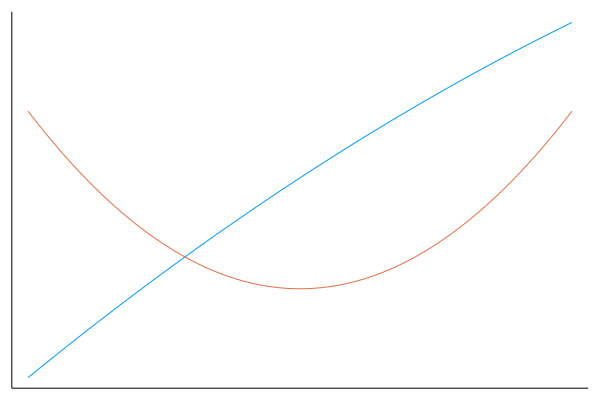
\includegraphics[scale=0.25]{images/bezint-1.png}}
  child{
    node [] {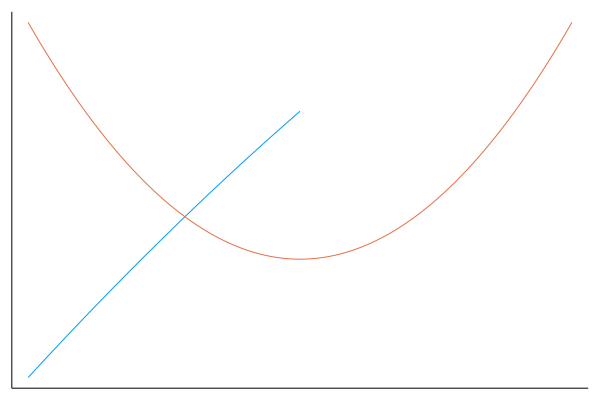
\includegraphics[scale=0.25]{images/bezint-2:1.png}}
    child{
      node [] {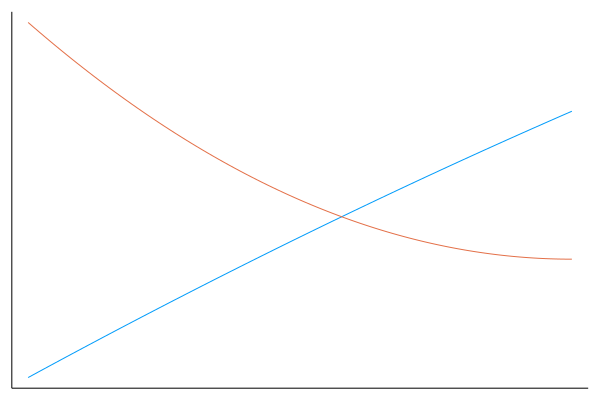
\includegraphics[scale=0.25]{images/bezint-3:1, 3.png}}
      %child{
      %  node [] {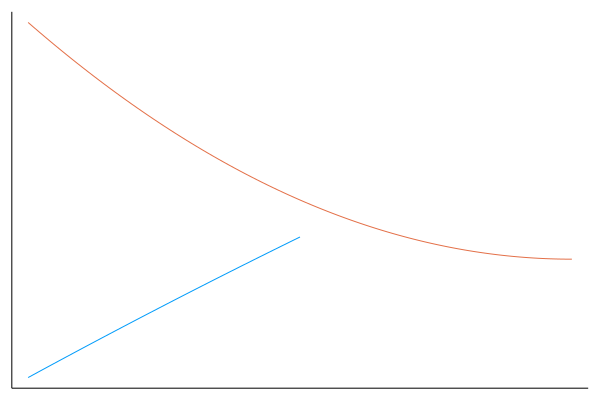
\includegraphics[scale=0.25]{images/bezint-4:1, 3, 1.png}}
      %  %child{
      %  %  node [] {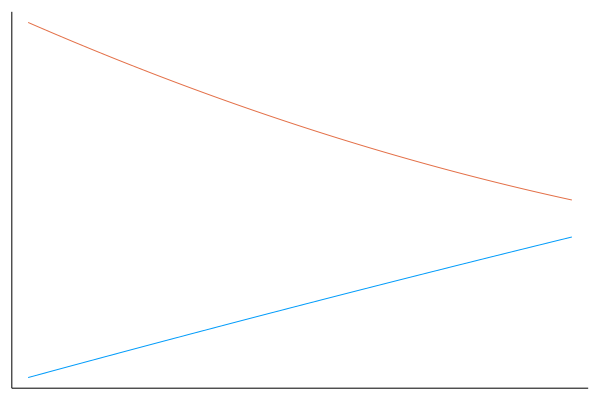
\includegraphics[scale=0.25]{images/bezint-5:1, 3, 1, 3.png}}
      %  %}
      %  %child{
      %  %  node [] {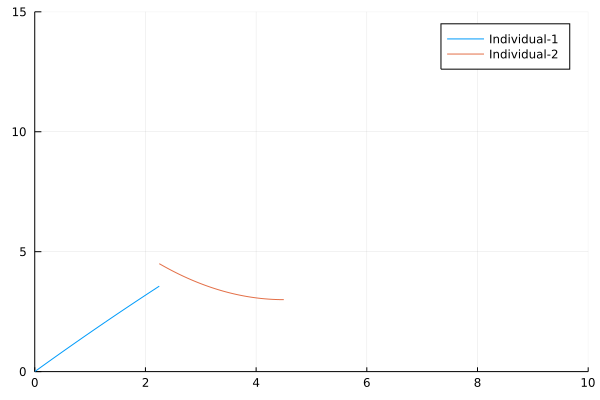
\includegraphics[scale=0.25]{images/bezint-5:1, 3, 1, 4.png}}
      %  %  child{
      %  %    node [] {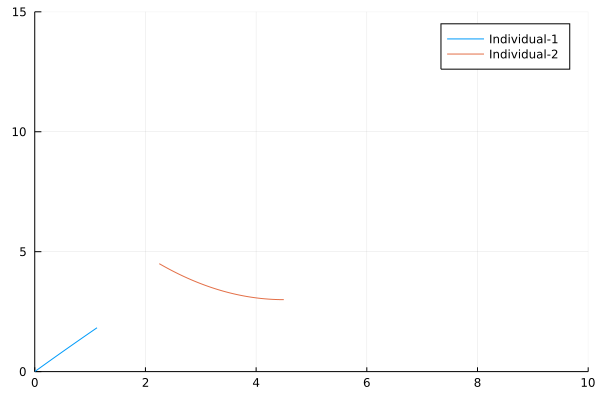
\includegraphics[scale=0.25]{images/bezint-6:1, 3, 1, 4, 1.png}}
      %  %  }
      %  %  %child{
      %  %  %  node [] {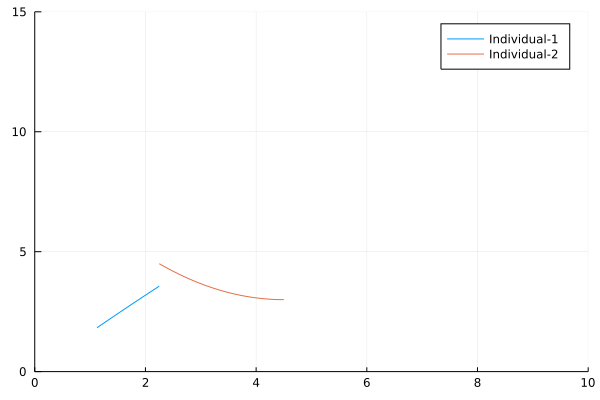
\includegraphics[scale=0.25]{images/bezint-6:1, 3, 1, 4, 2.png}}
      %  %  %  %child{
      %  %  %  %  node [] {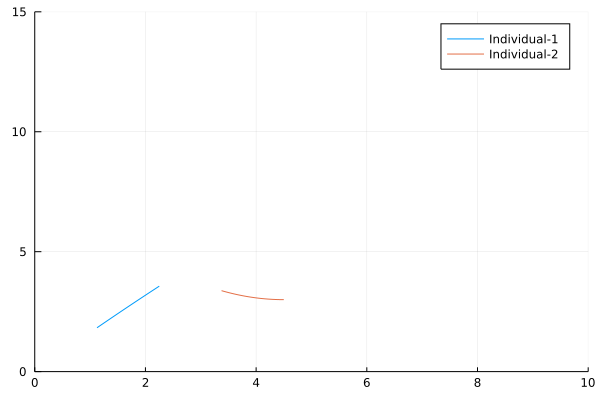
\includegraphics[scale=0.25]{images/bezint-7:1, 3, 1, 4, 2, 3.png}}
      %  %  %  %}
      %  %  %  %child{
      %  %  %  %  node [] {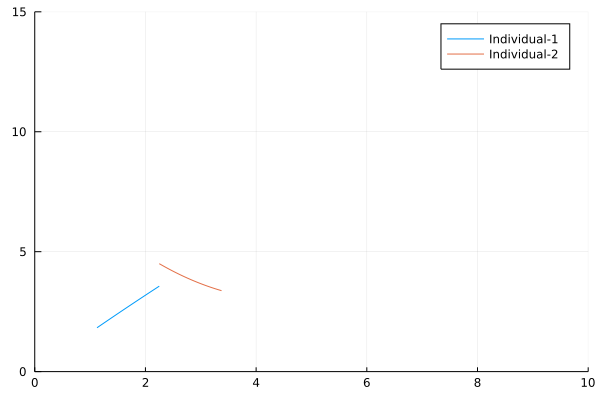
\includegraphics[scale=0.25]{images/bezint-7:1, 3, 1, 4, 2, 4.png}}
      %  %  %  %  child{
      %  %  %  %    node [] {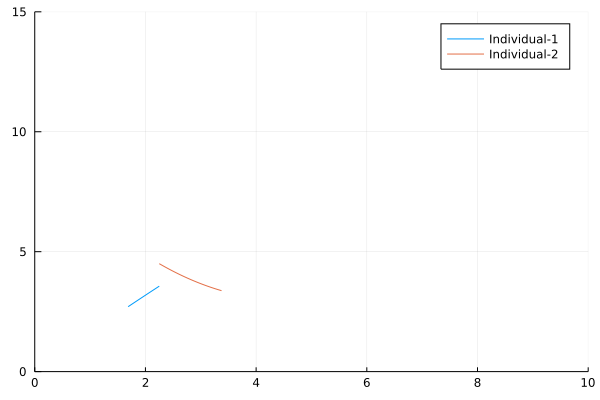
\includegraphics[scale=0.25]{images/bezint-8:1, 3, 1, 4, 2, 4, 1.png}}
      %  %  %  %  }
      %  %  %  %  child{
      %  %  %  %    node [] {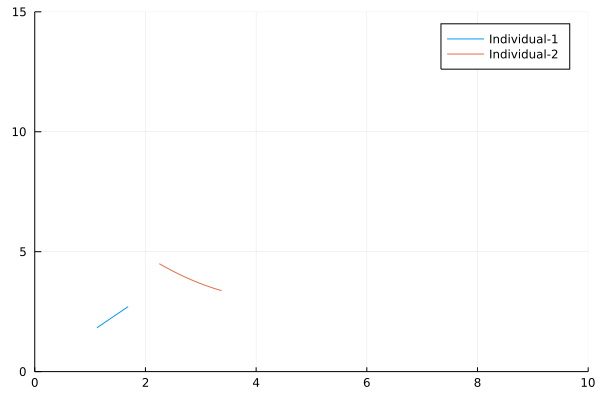
\includegraphics[scale=0.25]{images/bezint-8:1, 3, 1, 4, 2, 4, 2.png}}
      %  %  %  %  }
      %  %  %  %}
      %  %  %}
      %  %}
      %}
      %child{
      %  node [] {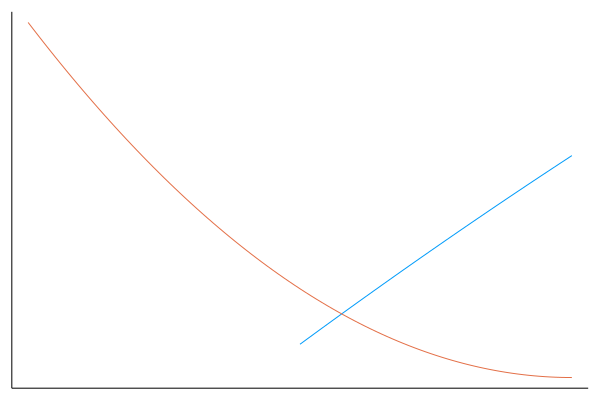
\includegraphics[scale=0.25]{images/bezint-4:1, 3, 2.png}}
      %  %child{
      %  %  %node [] {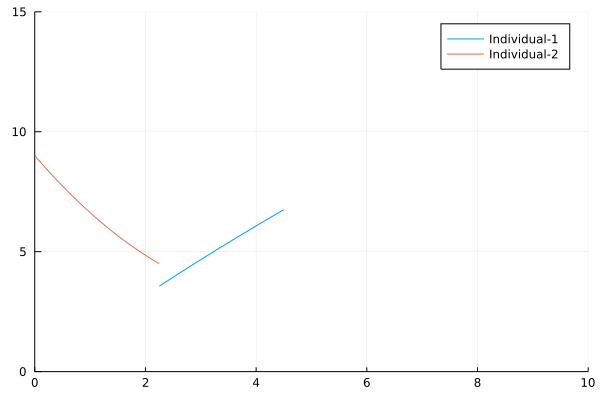
\includegraphics[scale=0.25]{images/bezint-5:1, 3, 2, 3.png}}
      %  %  %child{
      %  %  %  node [] {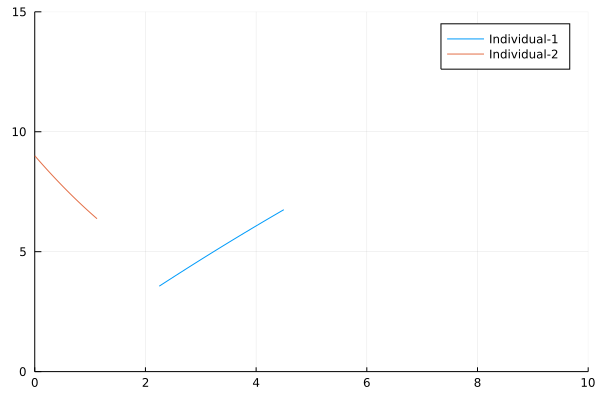
\includegraphics[scale=0.25]{images/bezint-6:1, 3, 2, 3, 3.png}}
      %  %  %}
      %  %  %child{
      %  %  %  node [] {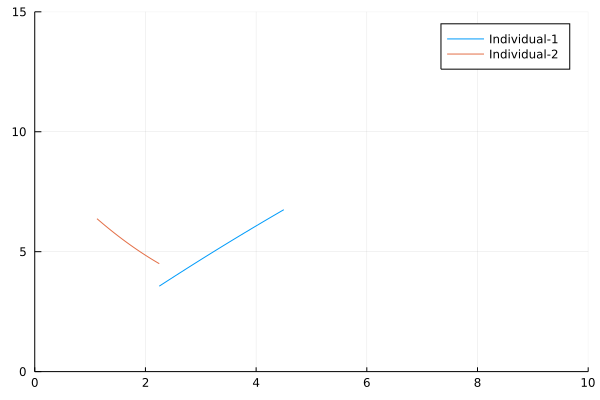
\includegraphics[scale=0.25]{images/bezint-6:1, 3, 2, 3, 4.png}}
      %  %  %  %child{
      %  %  %  %  node [] {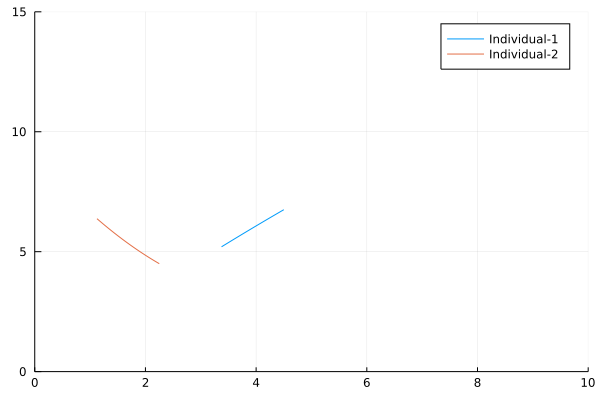
\includegraphics[scale=0.25]{images/bezint-7:1, 3, 2, 3, 4, 1.png}}
      %  %  %  %}
      %  %  %  %child{
      %  %  %  %  node [] {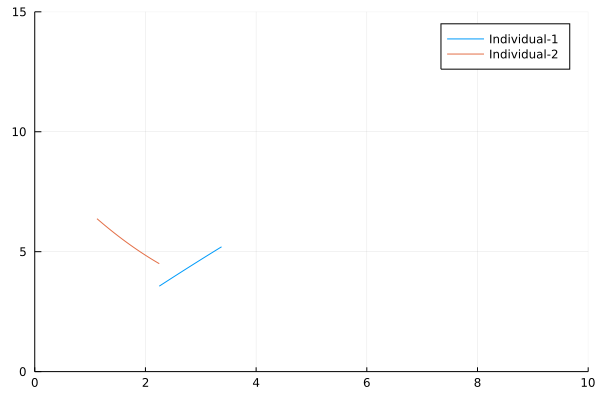
\includegraphics[scale=0.25]{images/bezint-7:1, 3, 2, 3, 4, 2.png}}
      %  %  %  %  child{
      %  %  %  %    node [] {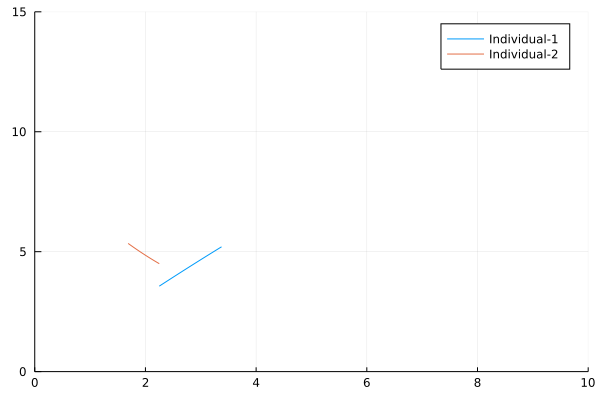
\includegraphics[scale=0.25]{images/bezint-8:1, 3, 2, 3, 4, 2, 3.png}}
      %  %  %  %  }
      %  %  %  %  child{
      %  %  %  %    node [] {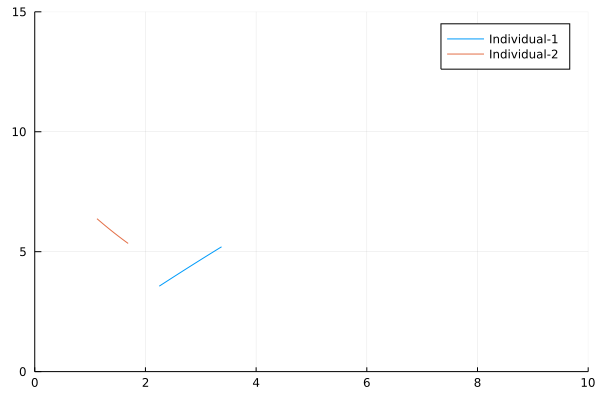
\includegraphics[scale=0.25]{images/bezint-8:1, 3, 2, 3, 4, 2, 4.png}}
      %  %  %  %  }
      %  %  %  %}
      %  %  %}
      %  %}
      %  %child{
      %  %  %node [] {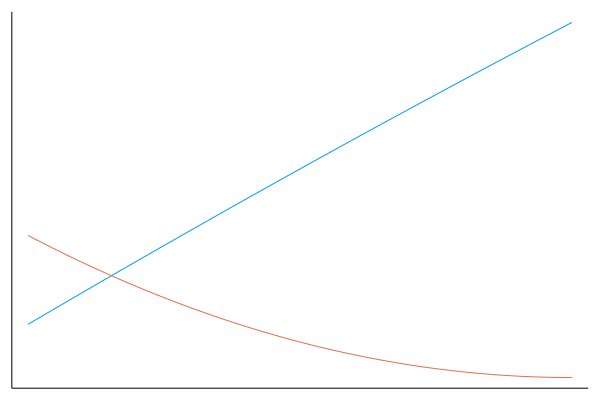
\includegraphics[scale=0.25]{images/bezint-5:1, 3, 2, 4.png}}
      %  %  %child{
      %  %  %  node [] {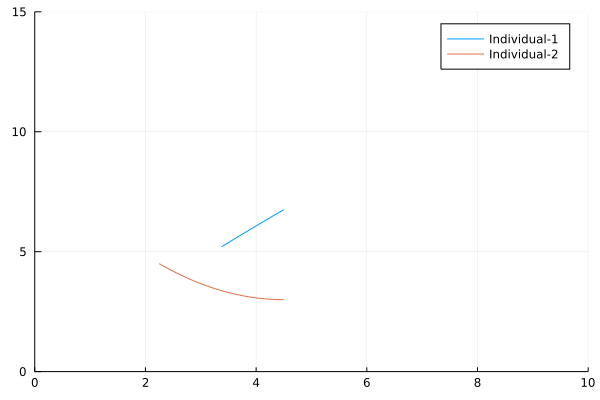
\includegraphics[scale=0.25]{images/bezint-6:1, 3, 2, 4, 1.png}}
      %  %  %}
      %  %  %child{
      %  %  %  node [] {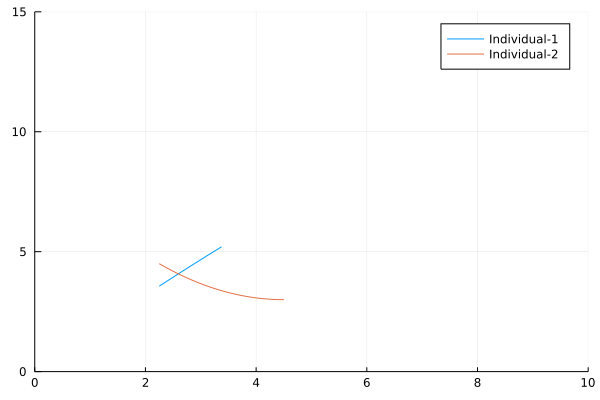
\includegraphics[scale=0.25]{images/bezint-6:1, 3, 2, 4, 2.png}}
      %  %  %  %child{
      %  %  %  %  node [] {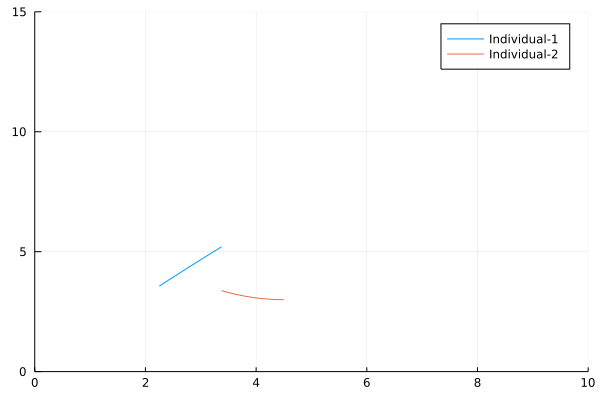
\includegraphics[scale=0.25]{images/bezint-7:1, 3, 2, 4, 2, 3.png}}
      %  %  %  %}
      %  %  %  %child{
      %  %  %  %  node [] {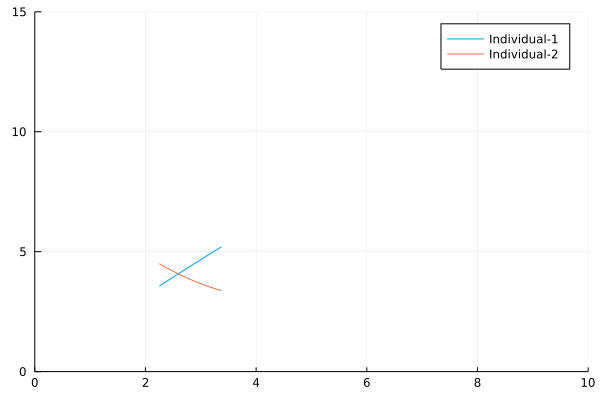
\includegraphics[scale=0.25]{images/bezint-7:1, 3, 2, 4, 2, 4.png}}
      %  %  %  %}
      %  %  %}
      %  %}
      %}
    }
    child{
      node [] {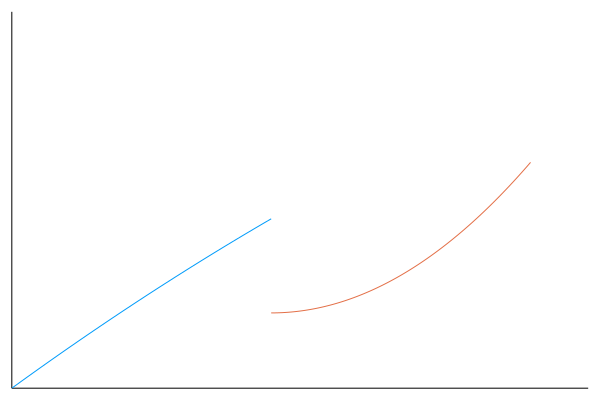
\includegraphics[scale=0.25]{images/bezint-3:1, 4.png}}
      %child{
      %  node [] {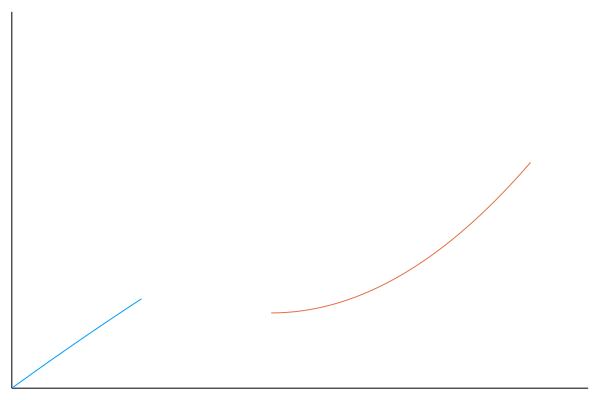
\includegraphics[scale=0.25]{images/bezint-4:1, 4, 1.png}}
      %}
      %child{
      %  node [] {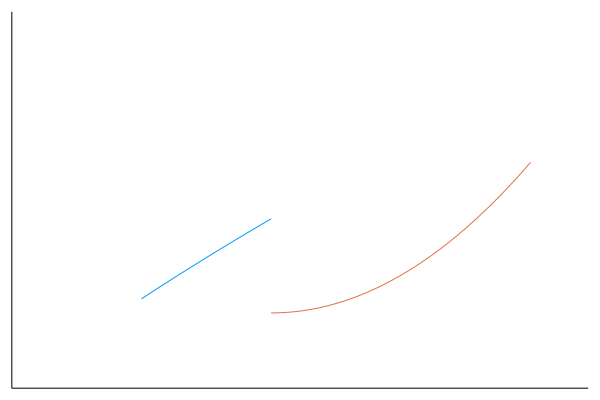
\includegraphics[scale=0.25]{images/bezint-4:1, 4, 2.png}}
      %  %child{
      %  %  %node [] {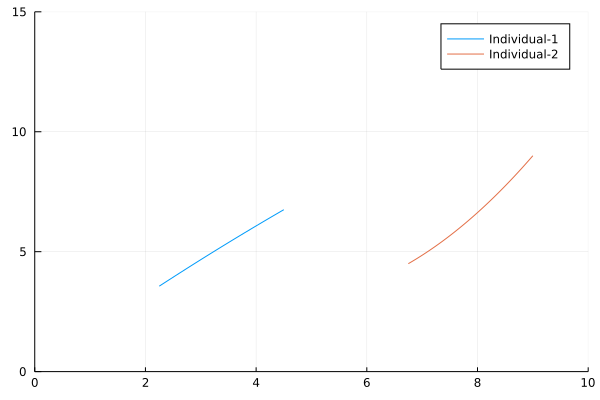
\includegraphics[scale=0.25]{images/bezint-5:1, 4, 2, 3.png}}
      %  %}
      %  %child{
      %  %  %node [] {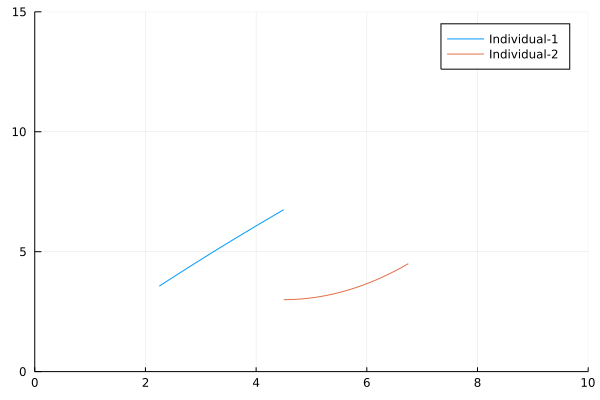
\includegraphics[scale=0.25]{images/bezint-5:1, 4, 2, 4.png}}
      %  %  %child{
      %  %  %  node [] {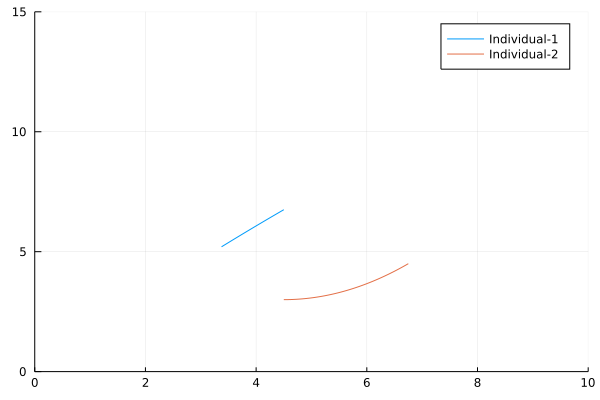
\includegraphics[scale=0.25]{images/bezint-6:1, 4, 2, 4, 1.png}}
      %  %  %}
      %  %  %child{
      %  %  %  node [] {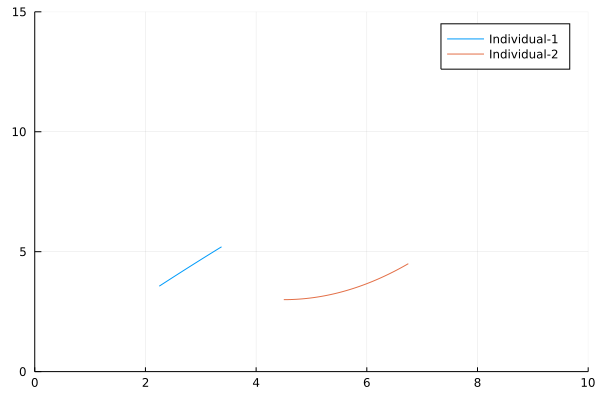
\includegraphics[scale=0.25]{images/bezint-6:1, 4, 2, 4, 2.png}}
      %  %  %}
      %  %}
      %}
    }
}
  child{
    node [] {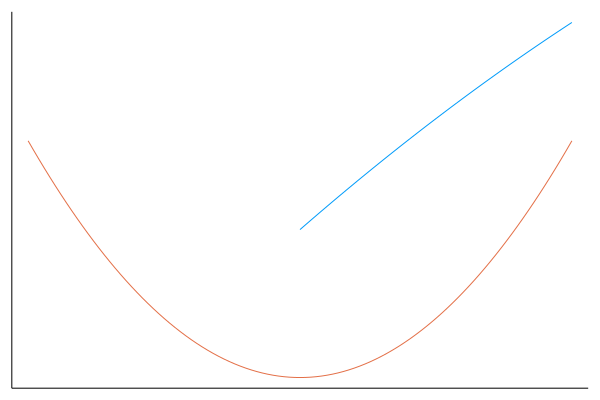
\includegraphics[scale=0.25]{images/bezint-2:2.png}}
    child{
      node [] {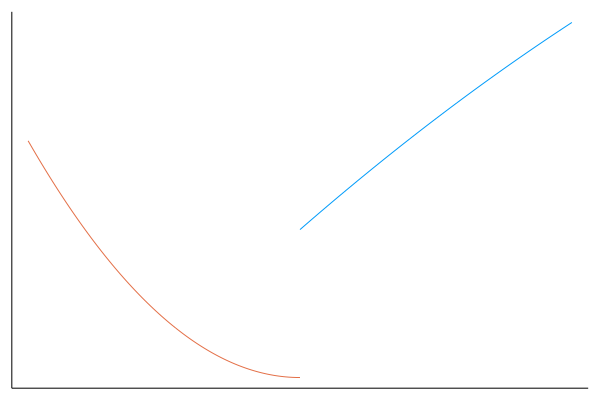
\includegraphics[scale=0.25]{images/bezint-3:2, 3.png}}
      %child{
      %  node [] {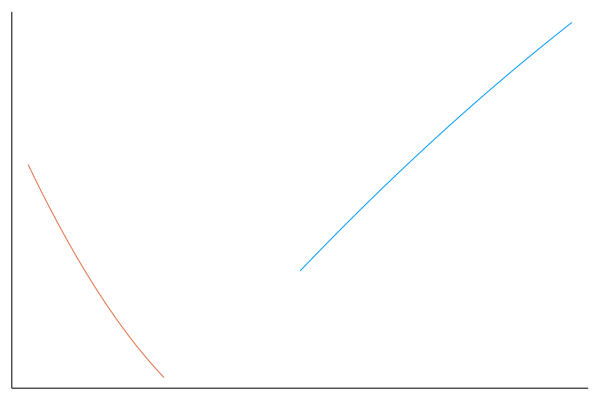
\includegraphics[scale=0.25]{images/bezint-4:2, 3, 3.png}}
      %}
      %child{
      %  node [] {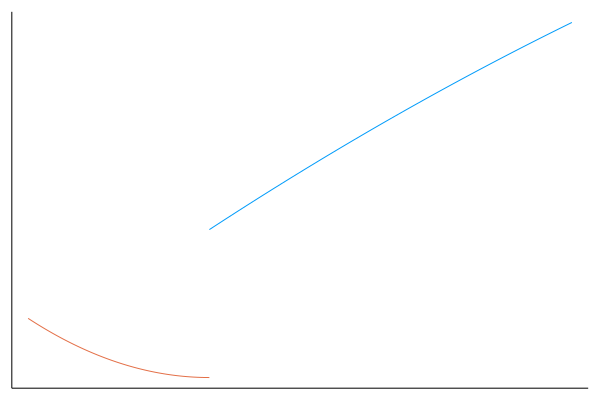
\includegraphics[scale=0.25]{images/bezint-4:2, 3, 4.png}}
      %}
    }
    child{
      node [] {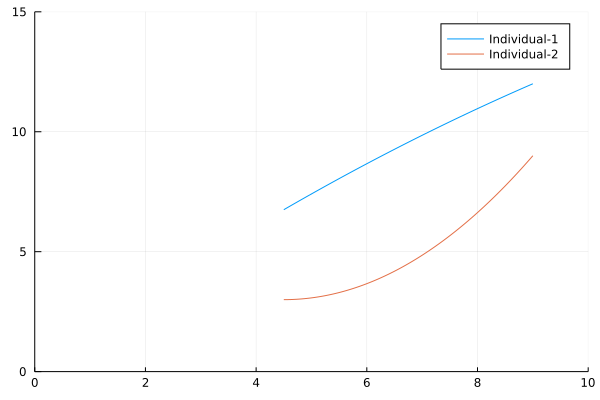
\includegraphics[scale=0.25]{images/bezint-3:2, 4.png}}
      %child{
      %  node [] {\includegraphics[scale=0.25]{images/bezint-4:2, 4, 3.png}}
      %  %child{
      %  %  %node [] {\includegraphics[scale=0.25]{images/bezint-5:2, 4, 3, 1.png}}
      %  %}
      %  %child{
      %  %  %node [] {\includegraphics[scale=0.25]{images/bezint-5:2, 4, 3, 2.png}}
      %  %  %child{
      %  %  %  node [] {\includegraphics[scale=0.25]{images/bezint-6:2, 4, 3, 2, 3.png}}
      %  %  %}
      %  %  %child{
      %  %  %  node [] {\includegraphics[scale=0.25]{images/bezint-6:2, 4, 3, 2, 4.png}}
      %  %  %}
      %  %}
      %}
      %child{
      %  node [] {\includegraphics[scale=0.25]{images/bezint-4:2, 4, 4.png}}
      %}
    }
  }
  ;

%  \node [below left = of p2-1] (p3-13) {\includegraphics[scale=0.25]{images/bezint-3:1, 3.png}};
%  \node [below right = of p2-1] (p3-14) {\includegraphics[scale=0.25]{images/bezint-3:1, 4.png}};
%
%  \node [below left = of p2-2] (p3-23) {\includegraphics[scale=0.25]{images/bezint-3:2, 3.png}};
%  \node [below right = of p2-2] (p3-24) {\includegraphics[scale=0.25]{images/bezint-3:2, 4.png}};


\end{tikzpicture}


\end{turn}
\caption{\label{fig:bezIntIllustration} Illustration of Bezier Intersection recursive subdivision method (Recursion depth =2)}
\end{figure}

\section{Macro-Level Planning} \todo{Title?}

The next stage in development is to attempt to implement the wrapper to solve Problem~\ref{prob:Spec} using the solution to Problem~\ref{prob:sub1}. I.e. to go from planning for multiple agents in a single section of road to planning for multiple agents across a network of interconnected roads.

\subsection{Road Graph Construction }

As specified in Problem~\ref{prob:Spec}, we require a description of the road space as a graph, $\mathcal{R}= (V,E)$ of intersections, $V$ and road segments $E$\todo[inline]{Should I define it as $\mathcal{R} = (I, R)$?}
.

This is a malleable definition allowing for a lot of information to be encapsulated whilst maintaining an abstract canonical description compatible with a swathe of mathematics through graph theory.\todo[inline]{wordy?}

I decided to use a mixture libraries to construct my road network: \texttt{Graphs.jl}\cite{JuliaAtticGraphsJl2021}, \texttt{LightGraphs.jl}\cite{Bromberger17}  and \texttt{SimpleWeightedGraphs.jl}\cite{JuliaGraphsSimpleWeightedGraphsJl2021}. The graph structures found in \texttt{Graphs.jl} allow for a lot of data (The entirety of the \texttt{Road} structure can be stored as edge metadata) to be encapsulated but do not offer the same functionality as those found in \texttt{LightGraphs.jl}, \texttt{SimpleWeightedGraphs.jl} utilises the \texttt{LightGraphs.jl} format but allows for weighted edges when applying the various standard graph-based algorithms (including Dijkstra), as such I created my own helper functions to convert between the two formats, which is a relatively simple process of filtering data into a new, more restrictive, structure.

In the simplified weighted digraph format, the edges are weighted by their length. Going forward it would be possible to incorporate more advanced heuristics into this, mimicking the method by which applications such as Google Maps plan routes. This could include congestion, road surface quality, known planned road obstruction such as maintenance or a predicted large influx of vehicles, for example the exodus of people from a large sports arena.

A visualisation of this format can be seen in Figure~\ref{fig:demoGraph} with edge names and their respective weights labelled.


\begin{figure}[ht]
  \centering
  \includegraphics[scale=0.4]{figures/demoGraph.png}
  \caption{\label{fig:demoGraph} Example Road Graph, edge names take the form $e$<start><end>: <edgeweight> }
\end{figure}


With the graph constructed the next stage is to plan what I will refer to as the \textit{macro} routes, i.e. the set of edges the agent must travel along $\{e_{1},\ldots,e_{m}\} \subseteq E$ to reach its destination intersection, $d \in V$.

\subsection{Macro-Route planning}

Macro-route planning, as described in Problem~\ref{prob:Spec}, is the process of taking a set of intersection pairs corresponding to agents and producing the set of edges which connect the vertex pairs in the shortest distance. This task is almost the exact specification for Dijkstra's algorithm~\cite{dijkstra1959note} for finding shortest paths in a connected digraph and as such this is the algorithm I employed to solve it.

The \texttt{LightGraphs.jl} library already implements this algorithm and the weighted element is incorporated by the \texttt{SimpleWeightedGraphs.jl} sub-library. As previously mentioned, the edges of my road-graph are weighted by their lengths.

For example the following construction of inputs for Problem~\ref{prob:Spec} over the graph seen in Figure~\ref{fig:demoGraph}:

\begin{align*}
  A &= \{ a_{1},a_{2},a_{3},a_{4} \} \\
  \mathcal{V} &= [ (1,4), (4,2), (1,4), (3,5) ]
\end{align*}

Would yield the following abstract routes for the agents:


\begin{align*}
  P &= \{ \\
  a_{1} &\mapsto \{ 1,3,2,5,4 \}, \\
  a_{2} &\mapsto \{ 4,5,2 \}, \\
  a_{3} &\mapsto \{ 1,3,2,5,4 \} ,\\
  a_{4} &\mapsto \{ 3,2,5 \} \\
          \}
\end{align*}

The next stage in the process is to group these agents into \textit{planning groups} i.e. groups in which agents will occupy the same road at the same time thus requiring cooperative planning.

\subsection{Agent Grouping}

When planning for multiple agents across multiple road spaces, routes may share the same stretch of road during route execution.

In the above example, it is trivial to see that agents $a_{1}$ and $a_{3}$ will share the same road at each stage of their route as they are following the same abstract path. We however, must also be able to determine whether agents $a_{1}$ and $a_{4}$ share road $e25$, it occurs in both of their routes but one agent may have left that stretch of road before the other enters.

This problem is solved using the algorithm seen in Algorithm~\ref{alg:pathgrouping}\feedback{do I need to make it more obvious that these algorithms are my own work? Are they clear enough?}
. For instance, on the example input above, we would expect to see the following grouping:

\begin{align*}
  (3,2) &\mapsto \{ \{ a_4,a_1,a_3 \}  \}, \\
  (4,5) &\mapsto \{ \{ a_2 \}  \}, \\
  (2,5) &\mapsto \{ \{ a_3,a_1 \}, \{ a_4 \}   \}, \\
  (5,2) &\mapsto \{ \{ a_2 \}  \} , \\
  (1,3) &\mapsto \{ \{ a_3,a_1 \}  \} , \\
  (5,4) &\mapsto \{ \{ a_3,a_1 \}  \}
\end{align*}

Where you can see $a_{4}$ occupies edge $e25$ at a time separate from agents $a_{1}$ and $a_{3}$.

\begin{algorithm}
  \caption{Path Grouping, \texttt{getPathGroupings} }\label{alg:pathgrouping}
  \KwIn{
  \begin{itemize}
    \item a road network graph $\mathcal{R} = (V,E)$
    \item a macro-path for each agent, $P$.
  \end{itemize}
}
Initialise map of roads, \texttt{roads}

\For{each road, $r \in E$}{
  \texttt{roads}[$r$] = [  ] \tcp*{Initialise list of agent groups}
}

\For{each agent's macro-path, $i \in P$}{
    Construct a running total of distance for each edge.

    \For{each edge, $e \in E$ in the macro-path}{

      \tcp*{Initialise routes sharing edge $e$ with agent $i$}
      microPlanAgents = [ i ]

      \For{each other agent's macro-path, $o \in P\backslash i$}{
        \If{$e \in o$ }{ \tcp*{routes $i$ and $o$ share an edge ($e$) at some point}

          \uIf{length of $i$ from origin to end of $e$ $>$ length of $o$ from origin to start of $e$}{
            \tcp*{routes $i$ and $o$ occupy the edge $e$ at the same time}
              append(microPlanAgents, o)
          }\Else{
            \tcp*{route $i$ exits edge $e$ before $o$ enters}
            continue
          }
        }
      }
      append(\texttt{roads}[$e$], microPlanAgents)
    }
  }

  \KwRet{roads}\tcp*{A map of edges to a list of lists of routes sharing that edge at the same time.}
\end{algorithm}

Once these grouping have been constructed, the next stage is to plan the low-level curves representing the paths each agent must take through each road segment, avoiding any agents it shares a given road segment with.

\subsection{Multi-agent route planning}\todo{title?}

This process is a wrapper around the previously implemented parallel planner described in~\ref{sec:maa}. It follows the algorithm outlined in Algorithm~\ref{alg:mrp}.

\begin{algorithm}
  \caption{Macro-route planner}\label{alg:mrp}
  \KwIn{
    \begin{itemize}
      \item set of start-goal pairs for each agent, $\mathcal{V}$
      \item a graph representing a road network, $\mathcal{R}$
    \end{itemize}
  }

  $P$ = $djikstraShortestPath(\mathcal{R},\mathcal{V})$

  pathGroupings = $\texttt{getPathGroupings}(\mathcal{R}, P)$

  routes = [] \tcp*{initialise routes array as list of paths through each road segment specified by macro-route in $P$}

  \For{each macro-path, $p\in P$}{
    \For{each edge $e \in p$}{
      concurrentAgentSets = pathGroupings[$e$]

      \For{concurrentAgents $\in$ concurrentAgentSets}{

        construct start and goal positions for each agent. This process requires further thought/ research \textbf{better way to talk about this?}

        paths = parallelPlanner(startPositions, goalPositions, $e$) \tcp*{Parallel planner, solution to Problem~\ref{prob:sub1}}

        \For{each agent $a_{i} \in \mathcal{V}$}{
          append(routes[$i$], paths[$i$])
        }

      }
    }
  }

  \Return{routes}

\end{algorithm}\todo{phrasing about s/e position calculation on alg~\ref{alg:mrp}}


My approach vastly simplifies the problem of intersection navigation and linking the routes between road segments, essentially assuming all road segments are sections of a single long road which line up exactly. Papers such as ``Automated Optimization of Intersections Using a Genetic Algorithm'' by Cruz-Piris et al.\cite{cruz-pirisAutomatedOptimizationIntersections2019} begin to tackle this problem through the use of cellular automata (building on the work of Maerivoet and De Moor\cite{maerivoetCellularAutomataModels2005}\todo[inline]{necessary?}
) and GAs (See Section~\ref{subsec:lit_rev-GACoopRoutes}) but substantial work would be required to link our two systems together.



\section{Language Choice}\todo[inline]{decide whether to remove this, I am thinking yes but last para is interesting, maybe move to evaluation}

I have chosen to implement my approach using the Julia language project\cite{JuliaProgrammingLanguage}.

Julia is a relatively new language first developed in 2012 by Jeff Bezanson, Stefan Karpinski and Viral Shah. It is a multi-paradigm language allowing for functional, object oriented (OO) and meta programming approaches to problems. I will mainly be using it for it's functional and OO capabilities.

Julia operates using multiple dispatch similar to languages such as Haskell. It interoperates with C and Fortran codebases without the need of middle-man bloat. This fact allows it to utilise the extensive high performance C libraries for floating point operations. Julia is eagerly evaluated, uses a Just in time compiler and has a garbage collector.

Julia features a syntax similar to both Python and Matlab with performance on par with C. As I am already very familiar with python and have studied functional programming in a number of modules; I found this language very quick and intuitive to learn and the resulting code to be clean, idiomatic and fast.

\todo{revise this para}A real-world deployment of a system based on my research would undoubtedly be required to run on small, relatively low performance, embedded systems and as such Julia may not be appropriate here. A language such as C or Rust may be used instead.

Julia also has distributed computation facilities. This sort of functionality could be extremely useful in a system such as mine as it could allow for computation to be spread across the agents themselves, removing the need for a central planning centre which could be a single point of failure.



%TC:macro \todo 1


%%% Local Variables:
%%% mode: latex
%%% TeX-master: "report"
%%% End:
